\documentclass{article}

% Language setting
% Replace `english' with e.g. `spanish' to change the document language
\usepackage[english,russian]{babel}
\usepackage{amsmath}

%графика
\usepackage{wrapfig}
\usepackage{graphicx}
\usepackage{pgfplots}
\usepackage{tikz}


\usepackage{tcolorbox}

% Set page size and margins
% Replace `letterpaper' with `a4paper' for UK/EU standard size
\usepackage[letterpaper,top=2cm,bottom=2cm,left=3cm,right=3cm,marginparwidth=1.75cm]{geometry}

% Useful packages
\usepackage{amsmath}
\usepackage{amssymb}
\usepackage{graphicx}
\usepackage{fixltx2e}
\usepackage[colorlinks=true, allcolors=blue]{hyperref}

\usepackage{geometry}
\geometry{left=25mm,right=25mm,
 top=25mm,bottom=25mm}

\title{Quantitative Analytics.\\
Lectures. Weeks 5-8. \\
Interest Rate Futures.}
\author{Andrey Lukianov}

% Колонтитулы
\usepackage{fancyhdr}
\pagestyle{fancy}
\renewcommand{\headrulewidth}{0.1mm}  
\renewcommand{\footrulewidth}{0.1mm}
\lfoot{}
\rfoot{\thepage}
\cfoot{}
\rhead{CMF-2022}
\chead{}

\begin{document}
\maketitle

% Оглавление
\setcounter{tocdepth}{1} % {2} - в оглавлении участвуют chapter, section и subsection. {1} - только chapter и section
\renewcommand\contentsname{Contents}
\tableofcontents
\newpage

% \section{Dictionary, Definitions, Abbreviations}

% \subsection{Dictionary}
% \begin{itemize}
%     \item IR - Interest rate - процентная ставка.
%     \item Compounding - платежи (idk)
% \end{itemize}

% \subsection{Definitions and Abbreviations}
% \begin{itemize}
%     \item SAR - Stated annual rate.
%     \item EAR - Effective annual rate.
%     \item FoC - Frequency of Compounding
%     \item PMT - Payment
%     \item r - Interest rate (at the moment). 
% \end{itemize}

\renewcommand{\labelitemi}{\tiny$\bullet$}
\renewcommand{\figurename}{Fig.}

 \section{Накопленный купонный доход}
 Фиксированные выплаты по облигации происходят в фиксированные моменты времени. 
 Однако мы можем посчитать так называемый \textbf{накопленный купонный доход(accrued interest)}, определяющий долю купона, накопленную на данный момент времени, считая с момента предыдущей выплаты.
 Для подсчета используется следующая формула:
 $$Accrued \enspace interest = coupon \frac{\text{количество дней, прошедших с последней купонной выплаты}}{\text{количество дней в купонном периоде}}$$
 Купонным периодом называют количество дней между между моментами времени, в которые происходят выплаты, coupon - размер регулярно выплачиваемого купона.
 
 \vspace{10mm}
 
 Для подсчета дроби, умножаемой на купон, используются различные \textbf{правила о подсчете дней(day count convention)}.
 
 В США наиболее популярны следующие 3:
 \begin{itemize}
     \item Казначейские облигации США(\textbf{US treasury bonds}) используют \textbf{actual/actual}: реальное количество дней, прошедшего с момента выплаты на реальное количество дней, между самой недавней выплатой и следующей после нее.
     \item Корпоративные и муниципальные облигации США(\textbf{US corporate and municipal bonds}) используют соглашение \textbf{30/360}. Это значит, что мы полагаем, что в году 360 дней(а значит, если в году выплат k, то промежуток между выплатами полагаем 360/k), а 30 означает, что мы считаем, что в месяце 30 дней и кол-во прошедших дней есть кол-во прошедших месяцев*30 + кол-во прошедших дней с начала месяца.
     \item Казначеские векселя(\textbf{US treasury bills}) используют подход \textbf{30/actual}, где \textbf{30} в числителе и \textbf{actual} в знаменателе  обозначают в точности то же самое, что и в прошлых пунктах.
 \end{itemize}
 
\begin{figure}[h]
\centering
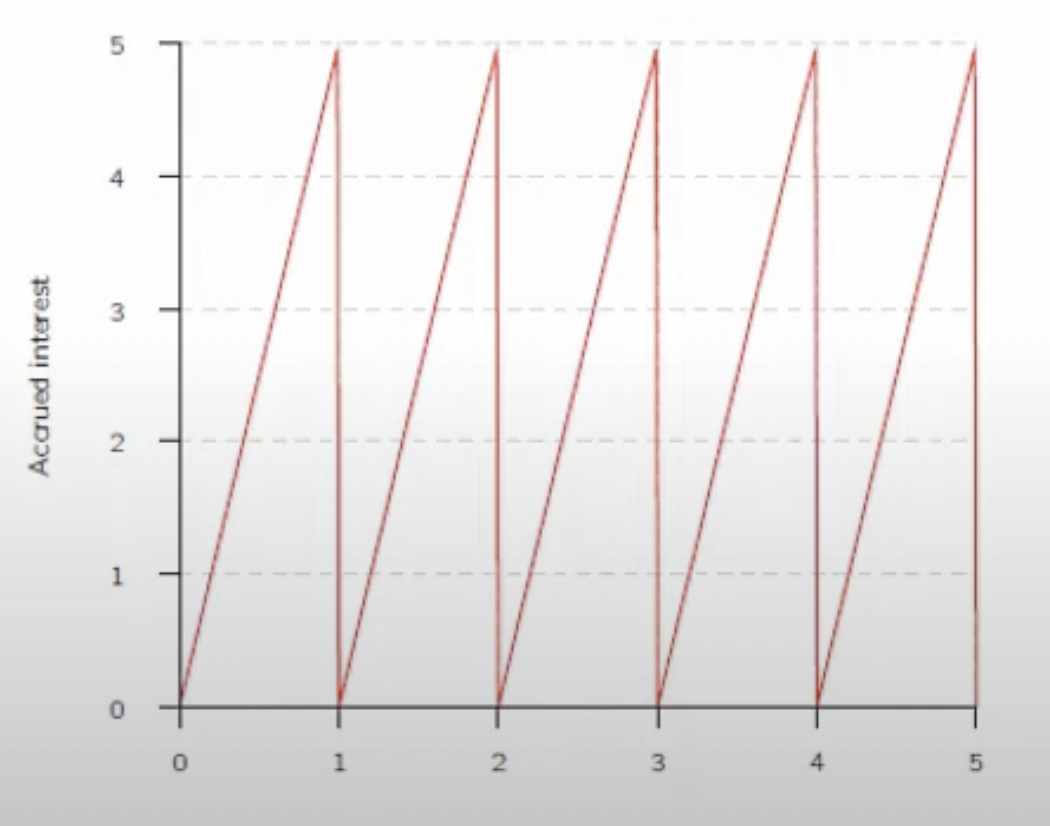
\includegraphics[width=0.7\textwidth]{accr_int.png}
\caption{Зависимость накопленного купонного дохода от времени. Важно, что после выплаты купона накопленный доход обнуляется и копится заново.}
\label{loadings}
\end{figure}

Пример: пусть есть облигация с полугодовыми выплатами и номиналом 100\$. Купоны выплачиваются 1 марта и 1 сентября. Годовая купонная ставка = 6\%. Сегодня 13 июля и необходимо посчитать купонный доход.
\begin{itemize}
    \item Для случая \textbf{actual/actual} мы получим, что между выплатами(от 1.03. до 1.09.) пройдет 184 дня, а между последней выплатой и данным моментом времени(от 1.03. до 13.07.) - 134 дня. Тогда накопленный купонный доход на 13 июля:
    $$\frac{134}{184}*100*\frac{6}{2} = 2.1848,$$ где процентная ставка делится на 2, поскольку выплаты производятся раз в полгода(два раза в год).
    \item Для случая \textbf{30/360} аналогичные рассуждения дадут:
     $$\frac{132}{180}*100*\frac{6}{2} = 2.2.$$
\end{itemize}
 

\section{Казначейские векселя и их расчет}

\textbf{T-bills(казначейские векселя)} рассчитываются и торгуются в терминах дисконтной ставки по соглашению о днях \textbf{actual/360}. Это считается некоторым аналогом купона, но купоном не является. Ставка, номинал и цена облигации(cash value) связаны следующим образом:
$$T-bills \enspace discount \enspace rate = \frac{360}{n} (100 - Y),$$ где Y - cash value, n - время до срока выплаты.
Заметим, что реальная доходность не совпадает с дисконтной ставкой, пример:
Пусть у нас есть казначейский вексель со сроком 0.5 года и годовой ставкой 5\%. Номинал равен 100\$. Найти ставку реальной доходности и стоимость векселя.


*\textbf{actual} для 0.5 года полагаем 180.

\begin{itemize}
    \item Наша годовая ставка 5\% и срок полгода дадут дисконтную ставку 5/2 = 2.5\% и купон 2.5\$ (100\$*0.05*$\frac{180}{360})$
    \item Cash Price: $Y = 100 - (T-bills \enspace discount \enspace rate)*n/360 = 100 - 5*180/360 = 97.5$
    \item Cтавка реальной доходности: $(100/Y - 1)*100 = (100/97.5 - 1)*100 =   2.564$
\end{itemize}

\section{Казначейские облигации и их расчет с учетом накопленного купона}
Специфика котирования \textbf{облигаций(T-bonds)} следующие: цена облигации записывается как: "число" "дробь", например, 95 5/32(это означает, что облигация стоит $95\frac{5}{32}\$.$ по отношению к 100 долларам. То есть облигация на 400 долларов будет стоить $95\frac{5}{32}*4 \$$ Дробь обычно измеряется в 32ых долях.
Поскольку по облигациям производятся выплаты, то Cash Price(цена облигации, по другому еще называют dirty price) = Quoted Price(котировка облигации(та самая 95 5/32), еще это называют present value of bond, либо чистой ценой(clean price)) + Accrued Interest(накопленный купонный доход)).
Еще раз, Cash Price = Quoted Price + Accrued Interest.


Пример:  пусть есть облигация с полугодовыми выплатами и номиналом 100\$. Купоны выплачиваются 1 марта и 1 сентября. Годовая купонная ставка = 6\%. Сегодня 13 июля и необходимо посчитать купонный доход. Пусть дополнительно эта облигация котируется как 102-11(то же самое, что 102 11/32). Требуется найти ее Cash Price.

\begin{itemize}
    \item Воспользуемся тем, что Quoted Price = 102 + $\frac{11}{32}$ = 102.34375
    \item Из задачи выше и определения о соглашении по датам для торговли облигации получим, что accrued interest = $\frac{134}{184}*100*\frac{6}{2} = 2.1848.$, заиспользовали \textbf{actual/actual} соглашение.
    \item Тогда Cash Price = 102.34375 + 2.1848 = 104.52855
\end{itemize}

\begin{figure}[h]
\centering
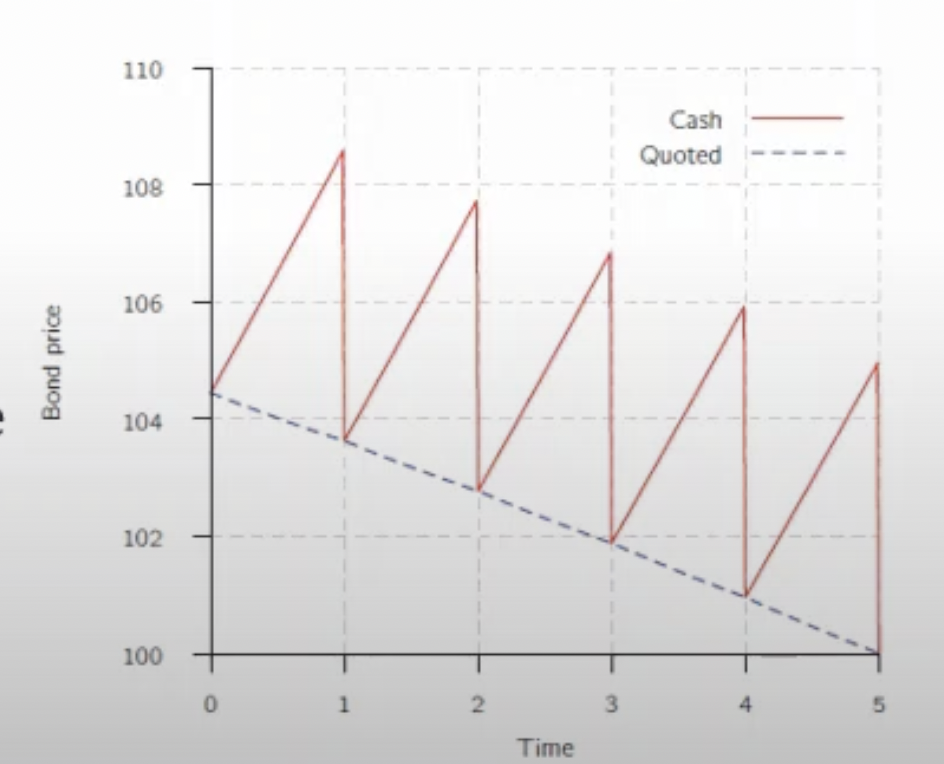
\includegraphics[width=0.7\textwidth]{acc_int_bond.png}
\caption{Стоимость облигации в зависимости от времени и накопленного купонного дохода.}
\label{loadings}
\end{figure}

\section{Фьючерсы на казначейские облигации США}
\begin{itemize}
    \item Здесь базовым активом служит не какой-то произвольный выпуск облигаций, а целый набор облигаций, дата погашения которых дальше на 15 лет от даты экспирации фьючерса.(То есть на момент поставки по фьючерсу облигации дата погашения этой самой облигации должна быть больше 15 лет)
    \item Таким образом, на самом деле под это условие подходит очень много облигаций
    \item Но возникает проблема по сравнению облигаций(купоны разные, даты экспирации тоже разные)
    \item Для уравновешивания облигаций по параметрам и приведения их параметрам к какому-то одному значению есть Conversion Factor(Конверсионный коэффициент). Обычно рассчитывают вот так:
    $$CF = \frac{\text{Present Value при постоянной кривой ставок 6\% - накопленный купонный доход}}{\text{номинал(face value)}}$$
    \item По этой формуле, если Present Value = 142, accrued interest = 2, face value = 100 , то CF = 1.4.
\end{itemize}

\section{Cheapest-to-Deliver bond}
Подсчет Сonversion Factor позволяет продающей стороне выбирать, какую облигацию положить в основу фьючерсного контракта для наибольшей прибыли.
При продаже облигации приток(Cash inflow) = QFP*CF + AI, где CF - conversion factor облигации, AI - accrued interest купона.
При этом отток(Cash outflow) = Quoted bond price + AI, где Quoted bond price - котировка облигации, по которой мы должны ее продать.
Тогда цель Cheapest-to-Deliver стратегии, это минимизировать Cash inflow - Cash outflow = QFP*CF - Quoted bond price, которая представляет из себя стоимость поставки облигации

Пример: в таблице приведены 4 облигации, которые будут продаваться с котировкой 95.75.
Найти наилучшую облигацию в смысле Cheapest-to-deliver. Получим, что наилучшая для этого облигация - облигация с номером 3.


\begin{figure}[h]
\centering
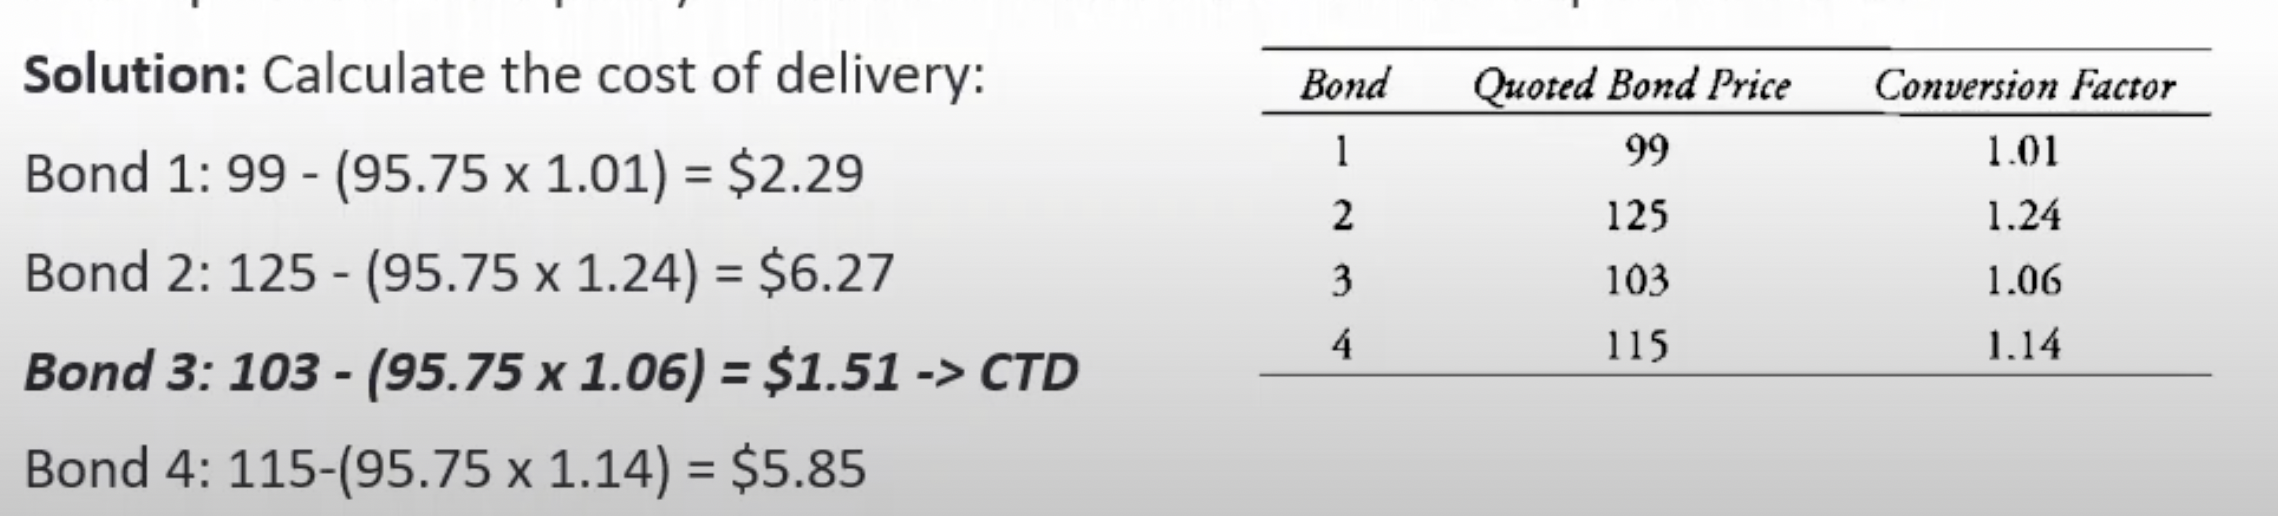
\includegraphics[width=0.7\textwidth]{cheap_to_del.png}
\caption{Предлагаемые для выбора облигации и решение задачи}
\label{loadings}
\end{figure}


Процедура выбора облигации предполагает большой перебор ценных бумаг, поэтому хотелось бы понимать, как Conversion Factor связан с реальной рыночной ситуацией(когда у нас не плоская 6\% ставка):
\begin{itemize}
    \item Если реальная ставка > 6\%, то Conversion Factor будет переоценивать бумаги и поэтому выгоднее взять облигацию с более долгим сроком и низким купоном.
    \item Если же наоборот реальная ставка < 6\%, то Conversion Factor будет недооценивать бумаги и стоит взять облигацию с менее долгим сроком и большим купоном.
    \item Если кривая ставок возрастает со временем, то выгоднее брать долгосрочные облигации.
    \item Если кривая ставок убывает со временем, то выгоднее брать краткосрочные облигации.
\end{itemize}

\section{Теоретическая фьючерсная цена}
Для обычного фьючерса имеем цену:
$$F_{0} = (S_{0} - I)e^{rT},$$
где $S_{0}$ - цена спота(Present Value), $I$ - сумма купонов, дисконтированных к сегодняшнему дню, $e^{rT}$ - капитализация к дате экспирации с процентной ставкой $r$.

Пример решения задачи на теоретическую фьючерсную цену:
Пусть есть казначейская облигация, выплачивающая 2 раза в год купон, c годовой процентной ставкой 10\%, Conversion Factor = 1.1, Quoted bond price = 100. Пусть в купонном периоде 180 дней и последний купон был выплачен 90 дней назад. Так же положим дату экспирации фьючерсного контракта 180 дней и безрисковую ставку дисконтирования 3\%.
\textbf{Решение}
\begin{itemize}
    \item Знаем, что Cash price = quoted bond price + accrued interest.
    \item Найдем accrued interest = coupon*$\frac{\text{days from last coupon}}{\text{days between coupons}}$ = $\frac{10}{2}\frac{90}{180}$ = 2.5
    \item Отсюда Cash price = 102.5
    \item Теперь нужно дисконтировать купон(получить I - present value купона). $I = coupon*e^{-rt} = 5*e^{-0.03*90/365}$
    \item Из формулы теоретической стоимости: $F_{0} = (S_{0} - I)e^{rT} = (102.5 - 4.96)*e^{0.03*180/365} = 98.99$
    \item Приведем к чистой цене: (QFP) = cash price - AI = 98.99 - 90/180*5 = 96.49
    \item Окончательно, применяя Conversion Factor, получим окончательную теоретическую стоимость: (QFP) = QFP*CF, отсюда QFP = 96.49/1.1 = 87.72
\end{itemize}

\section{Евродолларовые фьючерсы}
Не имеет отношения к курсу USD/EUR, это долларовый депозит, размещенный вне юрисдикции США.
По факту это договор о ставке, по которой мы можем разместить депозит 1млн \$ по 3х месячнойс ставке(LIBOR).

Этот контракт является расчетным, и изменение ставки на один базисный пункт(one basis point) соответствует 25\$ изменению на 1млн \$.

Исходя из этого, фьючерсный контракт оценивается следующим образом:
$$\text{eurodollar futures price} = 10000[100 - 0.25(100 - Z)],$$
где Z - котируемая цена облигации.
При Z = 97.8 цена контракта: 994500\$.


\begin{figure}[h]
\centering
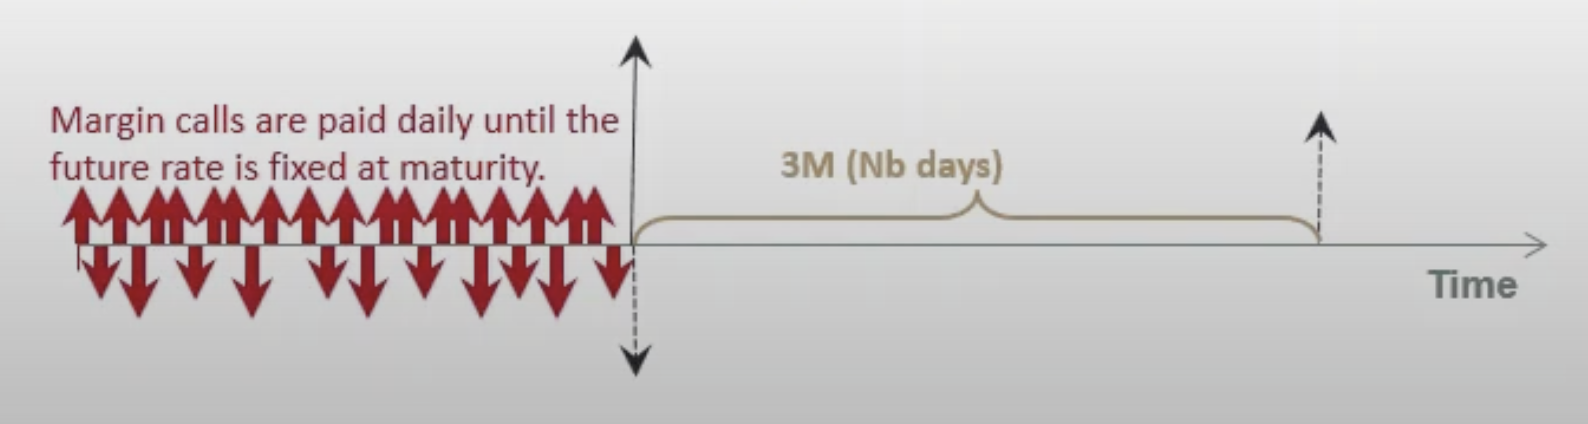
\includegraphics[width=0.7\textwidth]{eurusd.png}
\caption{Динамика евродолларового фьючерсного контракта}
\label{loadings}
\end{figure}

У этого контракта следующая механика: мы каждый день получаем приращение цены при изменении процентной ставки. В день экспирации мы фиксируем финальную ставку и, накапливаем  разницу между ценой покупки фьючерса и рыночной ценой на размещение денег в дату экспирации под 3 месяца.

Из-за этого возникает разница между ставками: фьючерсная ставка данного контракта получается выше, чем LIBOR, и тем разница больше, чем больше волатильна цена.

Если ставка идет вверх, то мы, как продающая сторона, начинаем зарабатывать, а если ставка идет вниз, то начинаем терять. Наблюдается некий эффект выпуклости, поэтому для подсчета реальной форвардной ставки используется поправка на выпуклость:
$$\text{actual forward rate} = \text{forward rate implied by futures} - \frac{1}{2} \sigma^{2}T_{1}T_{2},$$
где $\sigma$ - волатильность в 3х месячный период, $T_1$ - срок до экспирации фьючерса, $T_2 = T_1 + 90 \text{ days}$.

\section{Кривая процентных ставок по евродолларовым фьючерсам(LIBOR spot curve)}
Из формулы кривой по фьючерсам:
$R_{forward} = \frac{R_2 T_2 - R_1 T_1}{T_2 - T_1},$ где $R_i$ - ставка на горизонт $T_i$, то отсюда 
$$R_2 = [R_{forward}(T_2 - T_1) + R_1 T_1]/T_1,$$ где $R_2$ - ставка, посчитанная ранее по еврофьючерсным контрактам с учетом на выпуклость. Зная ставку и $T_1$, можем оценить на $T_2$, с $T_2$ на $T_3$ и так далее итерационно. 

\section{Хеджирование при помощи фьючерса на процентную ставку}
Duration-based hedge: хеджирование на основе дюрации.
Пусть у нас есть портфель с известной дюрацией(временем экспирации). Подбираем количество фьючерсных контрактов таким образом, чтобы суммарная дюрация стала нулевой:
$$N*F*D_{F} + P*D_{P} = 0,$$
где N - количество фьючерсных контрактов, F - цена фьючерса, $D_F$ - время экспирации фьючерсного контракта, P - цена портфеля, $D_P$ - время экспирации портфеля.

Недостатки такого хеджирования следующие:

\begin{itemize}
\item Не защищает от сильных изменений ставки(нелинейные изменения кривой ставки будут порождать большее отклонение в хеджировании).
\item Кроме того, кривая может изменяться по разному с разных сторон, а значит будет меняться и сама дюрация. На картинке представлено изменение хеджа, зависящее от изменения кривой ставки.
\end{itemize}

\begin{figure}[h]
\centering
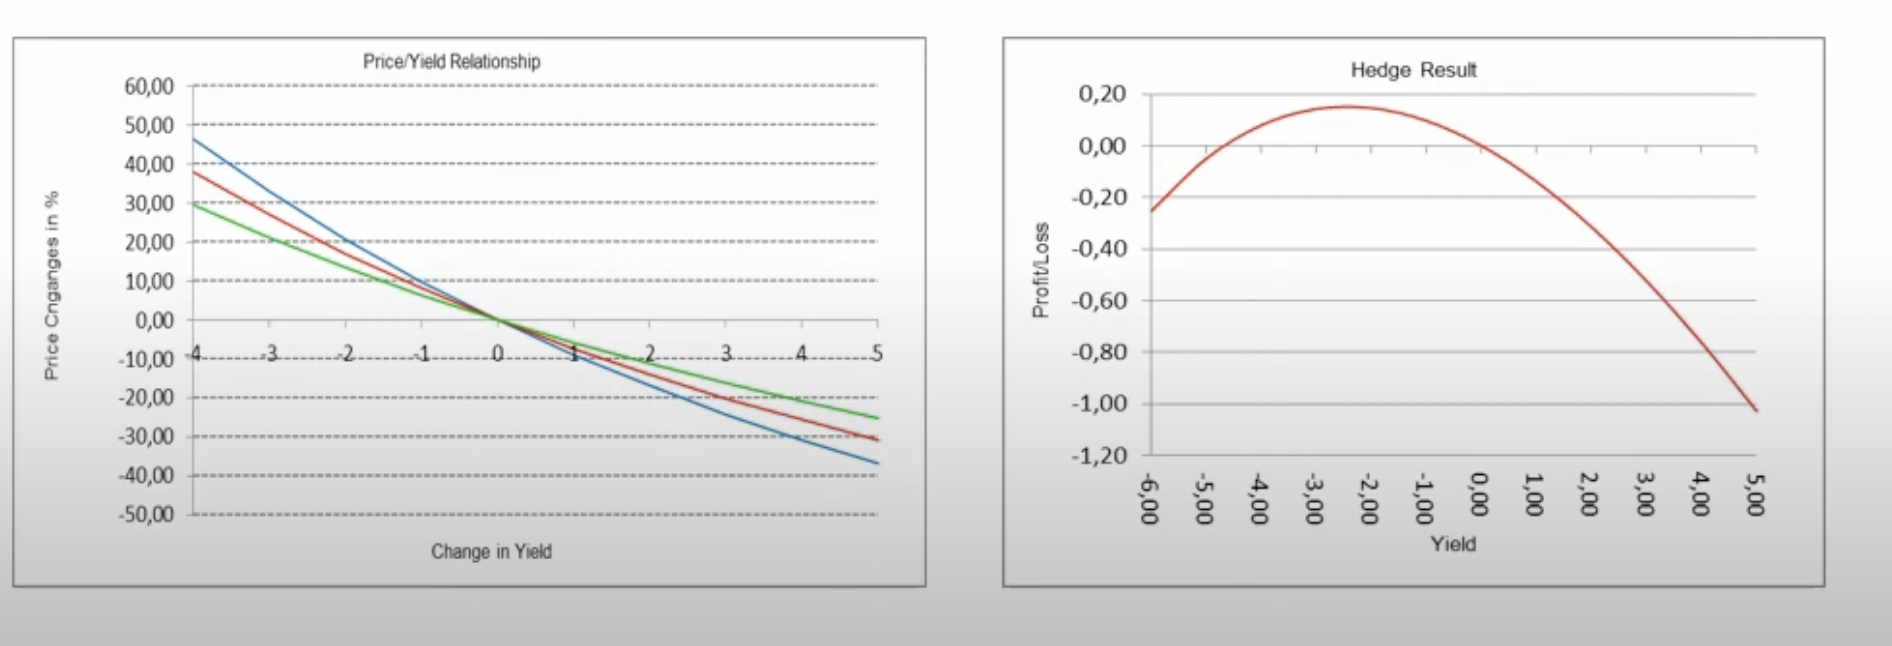
\includegraphics[width=0.7\textwidth]{yield_ch.png}
\caption{Чувствительность хеджа к изменению кривой ставок}
\label{loadings}
\end{figure}


\end{document}
